\documentclass[14pt,letterpaper,onecolumn]{scrartcl}
\usepackage{tocloft}
\usepackage{stdclsdv}
\usepackage{comment}
\usepackage{vmargin}
\usepackage{t1enc}
\usepackage{fancyvrb}
\usepackage{url}
\usepackage{calc}
\usepackage{array}
\usepackage{scrpage2}
\usepackage{graphicx}
\usepackage{color}
\usepackage{listings}
\usepackage[latin1]{inputenc}
\usepackage[english]{babel}
\usepackage{supertabular}
\usepackage{amssymb}
\usepackage{amsmath}
\usepackage{listings}
\usepackage{chicago}
\usepackage{truncate}
\usepackage{colortbl}
\usepackage{calc}
\usepackage{shortvrb}
\usepackage{fancybox}
\usepackage[pdftex,
            pagebackref=true,
            colorlinks=true,
            linkcolor=blue,
            pdfpagelabels,
            pdfstartpage=1
           ]{hyperref}
\pagestyle{scrheadings}
\usepackage[screen,nopanel,sectionbreak]{pdfscreen}
\margins{.2in}{.2in}{.2in}{.25in}
\screensize{4.5in}{6.5in}
\makeindex
\definecolor{LstColor}{cmyk}{0.1,0.1,0,0.025} 
\setcounter{tocdepth}{2}
\begin{document}
\setcounter{tocdepth}{2}
%%\frontmatter
\lstset{language=c++,basicstyle=\ttfamily\scriptsize,commentstyle=\ttfamily\small,tabsize=8,breaklines,backgroundcolor=\color{LstColor},fontadjust=true,keepspaces=false,fancyvrb=true,showstringspaces=false,moredelim=[is][\textbf]{\\emph\{}{\}}}

\title{Score Generation in Chord Spaces}
\author{
Michael Gogins  (michael.gogins@gmail.com)
}
\maketitle

\section{Musical Motivation}

\begin{itemize}
	
\item I am a composer, not a mathematician.

\item I like to use algorithms, e.g.\ fractals, that recursively generate a finished score in one pass.

\item Because current algorithms work in spaces without inherent musical significance, generated events must be mapped onto time and pitch.

\item Therefore, generated scores are often unstructured over larger scales of time and pitch.

\item It seems desirable to create algorithms that work directly with voice-leadings, chords, and so on.

\item The goal is neither to model music theory nor to reproduce existing styles, but simply to use generative procedures in spaces with some built-in musical semantics.

\end{itemize}

\section{Summary}

\begin{itemize}

\item The \emph{Tonnetz} is the graph of minimal voice-leadings between the major and minor triads. 

\item The \emph{Tonnetz} can be generalized as ``chord space,'' an orbifold (i.e.\ a quotient space) in which every point is a chord, and the smoothness of a voice-leading equals the closeness of its chords \cite{geometryofchords}. 

\item From chord space I derive related geometries to represent all trichords, higher arities of chord, voice-leading solutions, chord progressions, \emph{etc}. 

\item I present a Lindenmayer system that recursively rewrites an axiom by applying symbol replacement rules. The final production of the system is a string of commands for a turtle that moves within either a chord progression space, or a voice-leading space, to write a score.

\item I conclude by discussing other possibilities for score generators in mathematical spaces with built-in musical structure.

\end{itemize}

\section{Orbifolds}

\begin{itemize}

\item An \emph{orbifold} is a quotient space whose points are equivalent under a group action (any combination of translation, rotation, glide rotation, and reflection) that defines a symmetry. 

\item The group action permutes the corners of the orbifold, to glue faces of the quotient space together. 

\item For example, a strip of paper is a quotient space of the plane; gluing two ends together creates ring, which is an orbifold. 

\item Giving the ends a half twist before gluing them creates a Moebius band, another orbifold.

\end{itemize}

\section{\emph{Musical} Orbifolds}

\begin{itemize}

\item Music theorists distinguish various equivalence classes with respect to pitches: octave equivalence, permutational equivalence, inversional equivalence, and transpositional equivalence.

\item For each equivalence class, and each \emph{combination} of classes, there exists an orbifold in chord space. The equivalence defines which points of the space are identified to form the orbifold \cite{generalizedchordspaces}. 

\item The orbifold most familiar to musicians is pitch under octave equivalence, or pitch-class set space, $\textbf{R}/12\textbf{Z}$, where the octave is defined as 12 semitones.
	
\end{itemize}

\section{The \emph{Tonnetz} as Orbifold}

\begin{itemize}

\item Tymoczko and colleagues \cite{geometryofchords,generalizedchordspaces} are developing a geometric approach to music theory. Chords are represented as points in a linear \emph{chord space}, which has one dimension of pitch per voice, distinguishing inversions, octaves, and order of voices. This space extends up and down to infinity from a reference pitch at the origin. Chord space is continous, and every equally tempered and non-equally tempered chord can be defined in it.

\item \cite{geometryofchords} has identified the orbifold that divides pitch-class set space for $n$ voices by the symmetry group for $n$ voices: 

$\left(\textbf{R}/12\textbf{Z}\right)^{n}/\textbf{S}_{n}$. 

Its fundamental domains are $n - 1$ dimensional simplexes. 

\newpage

\item The points of the orbifold are identified by a group action that consists of a rotation (for odd numbers of voices) or a rotation plus a reflection (for even numbers of voices). Figure \ref{fig:tonnetzfortrichords} shows this orbifold for trichords. The lines connecting chords indicate movements of one semitone, so that joined chords are closest neighbors and the lines indicate all minimal voice-leadings. 

\begin{figure}[htbp]
	\centering
	  %trim left bottom right top
		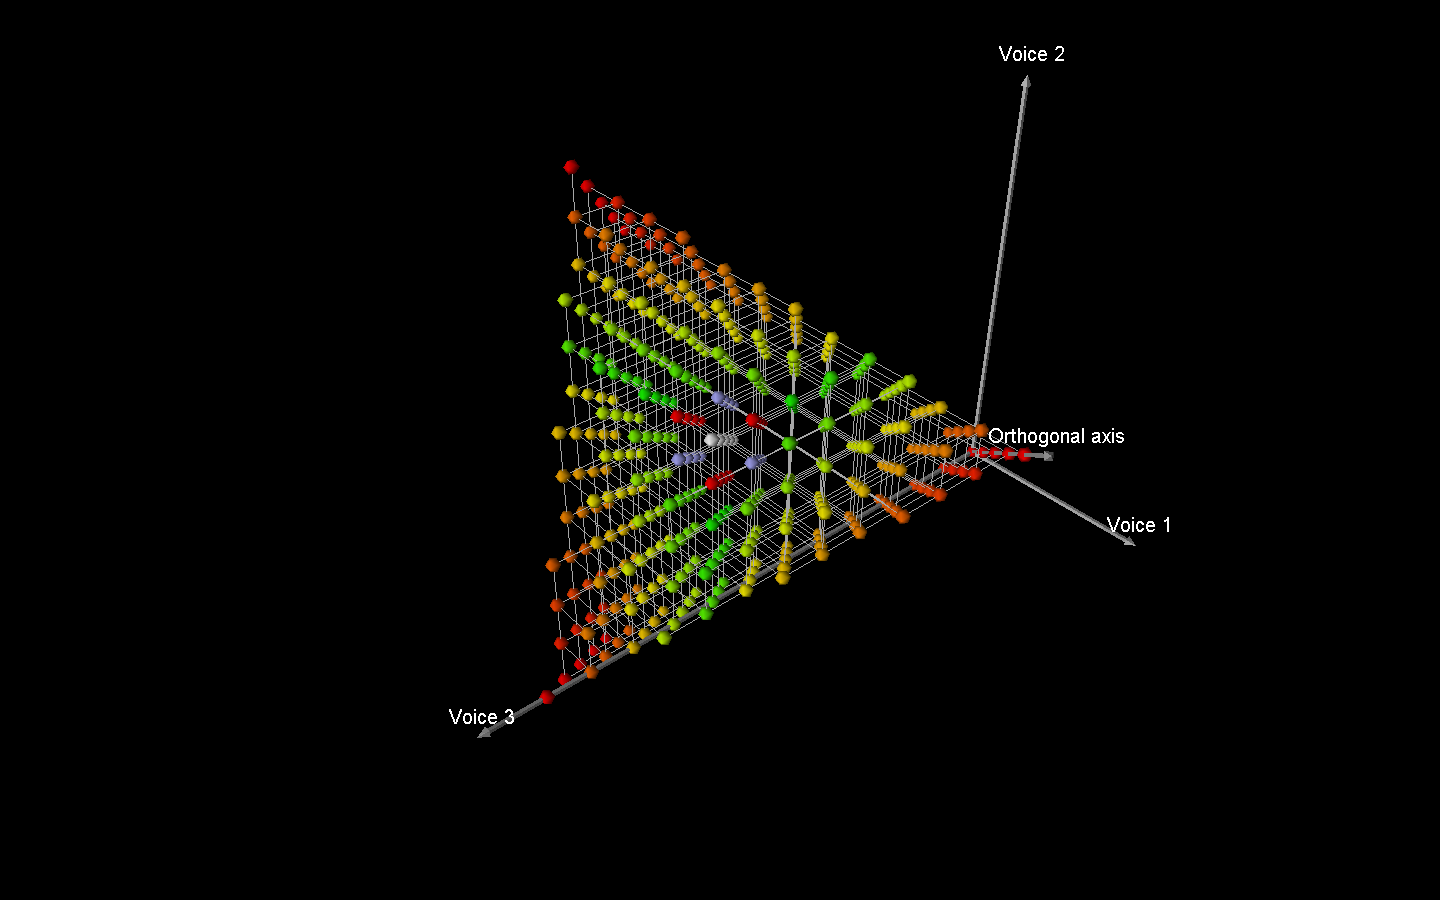
\includegraphics[trim=370 120 170 35,width=10cm,clip]{tonnetzfortrichords} 
	\caption{\textbf{\emph{Tonnetz} for trichords}}
	\label{fig:tonnetzfortrichords}
\end{figure}

\item The classical \emph{Tonnetz} of Oettingen, Euler, and Riemann is simply the six columns of major (red) and minor triads (blue) surrounding the central column of 4 augmented triads (white) that defines the orthogonal axis of symmetry of this orbifold. One end of the prism can also be visualized as being rotated $120 ^{\circ}$ and glued to the other end to form a torus.

\item As a geometric representation of the \emph{Tonnetz}, $\left(\textbf{R}/12\textbf{Z}\right)^{n}/\textbf{S}_{n}$ illuminates basic symmetries and constraints of Western music. 

\newpage

\item Within this orbifold, there is a one-to-one correspondence from voice-leadings to progressions between unordered pitch-class sets.

\item The major and minor triads are flexible with respect both to harmonic progression and to voice-leading because they not only surround the orbifold's axis of symmetry, but also lie near each other. Similarly, for tetrachords, commonly used seventh chords surround the orthogonal column of diminished seventh chords. 

\end{itemize}

\section{Scores and Operations}

\begin{itemize}

\item The present work represents musical scores as functions of time onto chord space. Arpeggios, passing tones, counterpoint, etc.\ are represented as succcessions of more or less fleeting chords.

\item Chord spaces themselves are not sufficient to serve as spaces for composing:

\begin{itemize}

\item For automatic score generation it is necessary to represent octaves, which breaks the octave equivalence of the \emph{Tonnetz}.

\item Whereas a primitive operation such as a translation vector that does not cross a face of the orbifold has of course always the same orientation, if the same translation \emph{does} cross a face, it can change orientation as it is reflected from a symmetry hyperplane. It is easier to visualize progressions in spaces in which there are no mirrors, so that (for example) adding a vector to a chord always moves it along the same orientation.

\end{itemize}

\end{itemize}

\section{Variations on Chord Space}

\begin{itemize}

\item Consequently, I have found the following variations on chord space to be useful for primitive operations in score generation: 

\begin{description}
	
\item[Ranged chord space] Chord space for $n$ voices under equivalence for range $R$ defines the orbifold $\left( \textbf{R}/R\textbf{Z}\right)^{n}$. Voices that move past the top of the range re-appear at the bottom. Figure \ref{fig:rangedchordspace} shows ranged chord space for 3 voices. Because its opposing faces are identified, the cube is actually a 3-dimensional torus.

\begin{figure}[htbp]
  \begin{center}
	  %trim left bottom right top
		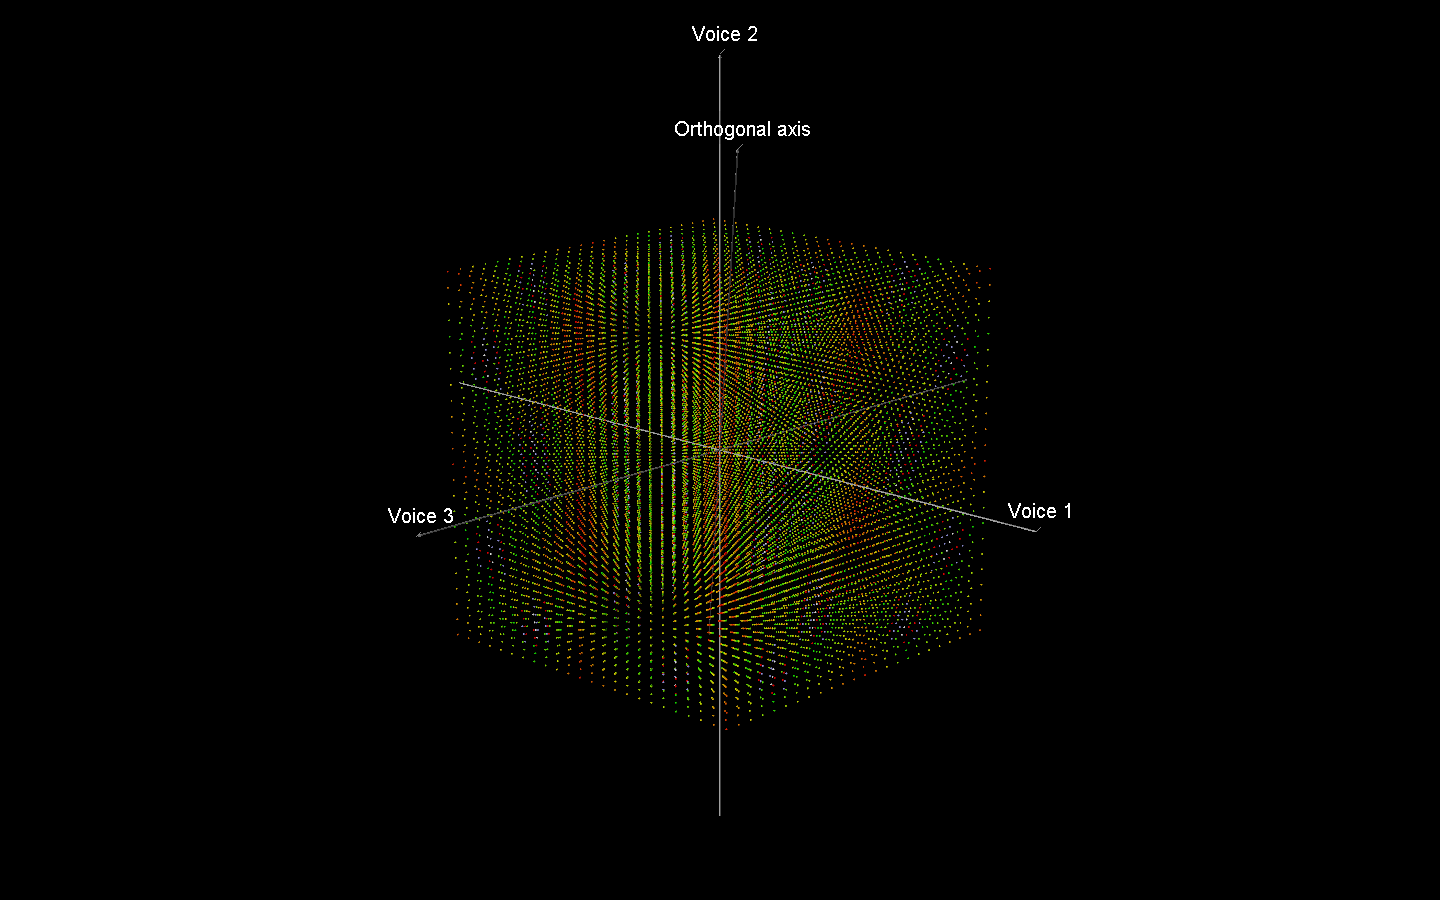
\includegraphics[trim=290 80 270 0,width=8.5cm,clip]{rangedchordspace} 
	\caption{\textbf{Ranged chord space for 3 voices, 2 octaves}}
	\label{fig:rangedchordspace}
  \end{center}
\end{figure}

\item[Normal chord space] This space can be formed by dividing the fundamental domains of the completed \emph{Tonnetz} into symmetrical ``kites'' and stacking them on top of each other, as shown in Figure \ref{fig:normalchordspace} for trichords. The column is formed by the inversion of each chord that is closest to the orthogonal axis. This is related to, but not the same as, the theoretical notion of ``normal form.''

\begin{figure}[!htp]
	\centering
	  %trim left bottom right top
		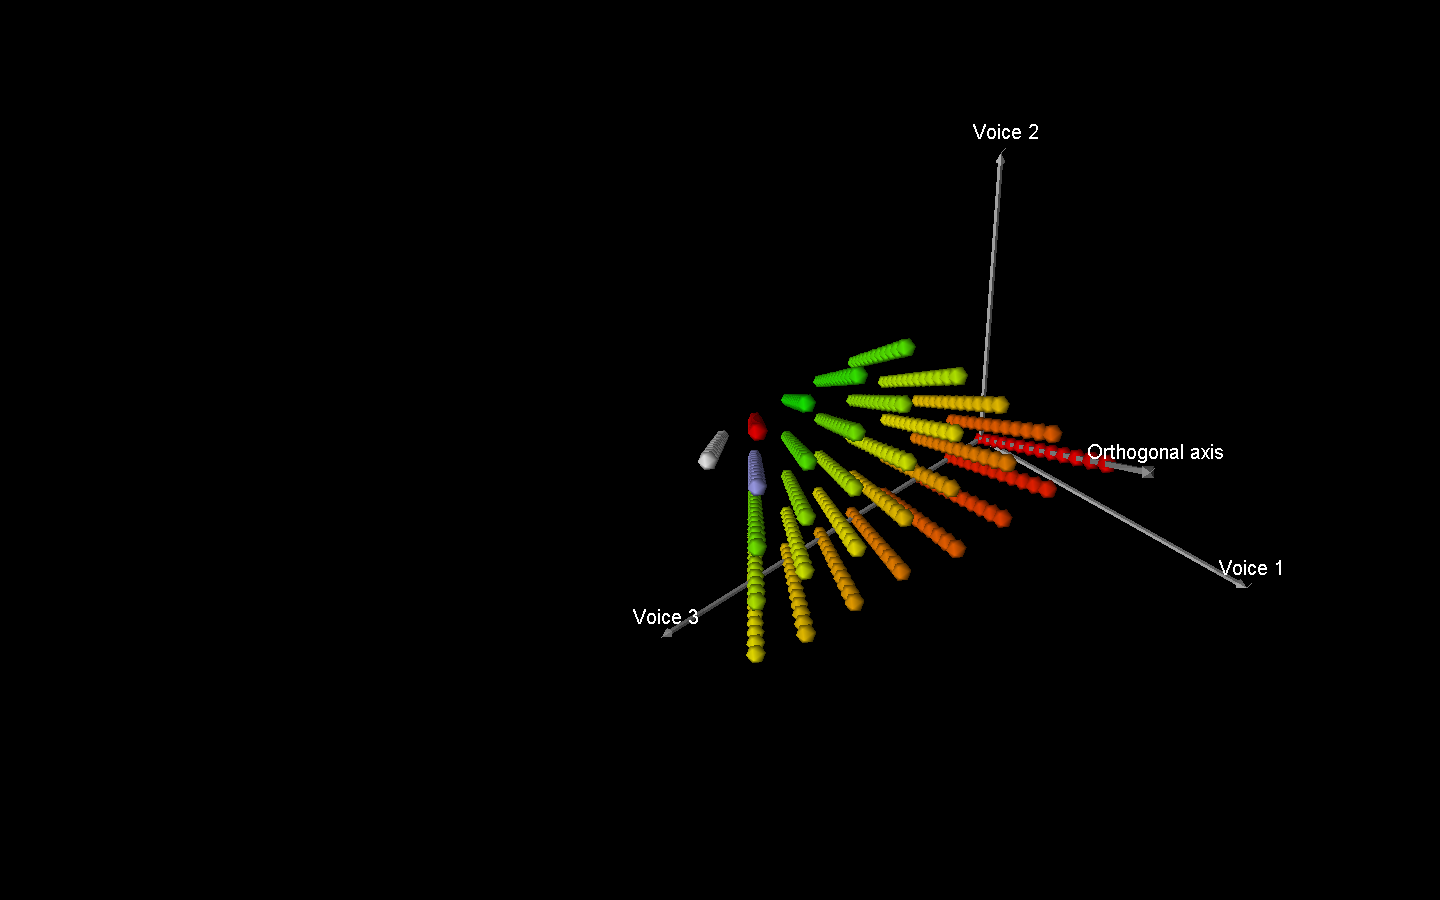
\includegraphics[trim=565 220 100 110,width=10cm,clip]{normalchordspace} 
	\caption{\textbf{Normal chord space for trichords}}
	\label{fig:normalchordspace}
\end{figure}

\end{description}

\end{itemize}

\section{Voice-Leading in Ranged Chord Space}

\begin{itemize}

\item Tymoczko defines a normlike total preorder for voice-leadings within chord spaces, first by smoothness (distance between chords, using either the taxicab norm or the Euclidean norm), and then by parsimony (fewer or shorter movements of voices). Every known measure of voice-leading size creates a normlike total preorder \cite{geometryofchords}.

\item I have used this normlike ordering to implement a simple algorithm for finding the closest voice-leading in ranged chord space from a source chord to a target pitch-class set. Such algorithms can be very useful in score generators. Keep in mind that each voice of the source chord could be in any octave of the space's range. As both the octave-equivalent and ranged chord spaces inherit their metric from the same parent, Euclidean space, it follows that the normlike total preorder for voice-leadings also exists in ranged chord space.

\subsubsection{Voice-Leading Algorithm}

\begin{enumerate}

\item Store the source chord and target pitch-class set.

\item Generate the lattice of all chords within ranged chord space that match the target pitch-class set, by iterating octavewise through all points in the space.

\item Compare the voice-leading from the source chord to each chord in the lattice, first by smoothness, then by parsimony (it is easy to add the option of excluding parallel fifths). 

\item Return the target chord with the closest voice-leading.

\end{enumerate}

\item My current implementation performs a brute force search to compare voice-leadings, but as long as this need not be done in real time, it is quite fast enough. 

\end{itemize}

\section{Lindenmayer Systems}

\begin{itemize}

\item A Lindenmayer system consists of an axiom (initial string of atoms), some rules each specifying how one atom is to replaced with a string of atoms, an implicit rule that an atom with no replacement is replaced by itself, and the number of iterations for the recursion \cite{algorithmicbeautyofplants}. 

\item Some atoms are commands for a ``turtle'' in a drawing system. \texttt{F} might mean move one step while drawing a line, \texttt{f} move one step without drawing a line, \texttt{+} turn right, \texttt{-} turn left, \texttt{[} push the turtle state onto a stack, and \texttt{]} pop the turtle state from the stack. 

\item Repeated replacements usually expand the initial axiom into a long string of atoms --- the \emph{production} of the system. 

\item This is then interpreted as a program for the turtle, which draws a figure in the space. 

\end{itemize}

\subsection{$OL$ Lindenmayer Systems}

\begin{itemize}

\item In the simplest type of Lindenmayer system, or $OL$ system, the replacement rules do not depend on the state of the production on either side of the current atom, and take no parameters. 

\item $OL$ systems have been used for some time to generate musical scores in spaces where time is one dimension of the space \cite{usinggenerativegrammarsformusiccomposition,fractalmusicwithstringrewritinggrammars,grammarbasedmusiccomposition}.

\item I adapted $OL$ systems to generate scores in chord spaces where each dimension is a voice, and time is simply the sequence of chords. 

\item I implemented the score generator using Python \cite{python}, the SciPy package which provides efficient matrix arithmetic for Python \cite{scipy}, and CsoundVST, an extended version of Csound 5 with Python scripting and some facilities for mathematically-based algorithmic composition \cite{csoundmanual}.

\end{itemize}

\subsection{An $OL$ Lindenmayer System for Musical Orbifolds}

\begin{itemize}

\item The turtle is a position vector in $n$-dimensional chord space, the step is another vector, movement adds the step to the turtle, the step can be multiplied by a rotation matrix to point in a new direction. 

\begin{itemize}

\item Sometimes the turtle is moving voicewise in ranged chord space (\texttt{V} commands), or voice-leading space.

\item Sometimes the turtle is moving chordwise in normal chord space (\texttt{P} commands), or chord progression space. 

\item Chords are created with the \texttt{C} commands. 

\begin{itemize}

\item The \texttt{Ca} command creates a chord at the current absolute position of the turtle in ranged chord space. 

\item The \texttt{Cv} command creates a chord with the target pitch-class set, but the voice-leading that is closest by Tymoczko's measure, using the algorithm described above.

\end{itemize}

\end{itemize} 

\item Because each operation is defined on one or another quotient of chord space, all operations can actually be performed on points in chord space alone, using ordinary matrix arithmetic. The actual quotient space is defined by applying a specific modulus or some other action that identifies points in the space. 

\item Time is defined as the sequence of chords, and the turtle state includes the size of the time step (\texttt{T} commands). The paper contains the complete table of turtle commands.

\end{itemize}

\newpage

\subsection{A Musical Example}

\begin{itemize}

\item The \texttt{Pv} and \texttt{Cv} turtle commands shown in Table \ref{tab:progression1} set up a C major 7$^{th}$ chord, then create a IM7 ii7 V7 VIM7 progression (Figure \ref{fig:progression1}). 

\begin{table}[htbp]
\begin{tabular}{l|p{12cm}}
\hline
Iterations & 1\\
Axiom & \ttfamily C=CM7 Cv Pv1,2,1,2 Cv Pv5,5,5,6 Cv Pv2,2,3,2 Cv \\
\hline
\end{tabular}
\caption{\textbf{Progression}}
\label{tab:progression1}
\end{table}

\begin{figure}[htbp]
	\centering
		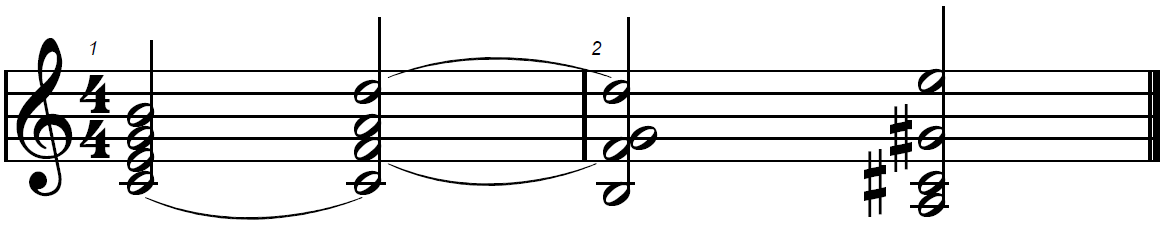
\includegraphics[width=8.5cm]{progression1}
	\caption{\textbf{Progression}}
	\label{fig:progression1}
\end{figure}

\item A sequence of these progressions can be created using a simple Lindenmayer system with one substitution rule (Table \ref{tab:sequence}, Figure \ref{fig:sequence}). 

\begin{table}[tbp]
\begin{tabular}{l|p{12cm}}
\hline
Iterations & 1\\
Axiom & \ttfamily C=CM7 A A A \\
Replace \ttfamily A & \ttfamily Cv Pv1,2,1,2 Cv Pv5,5,5,6 Cv Pv2,2,3,2 Cv\\
\hline
\end{tabular}
\caption{\textbf{Sequence}}
\label{tab:sequence}
\end{table}

\begin{figure}[htbp]
	\centering
		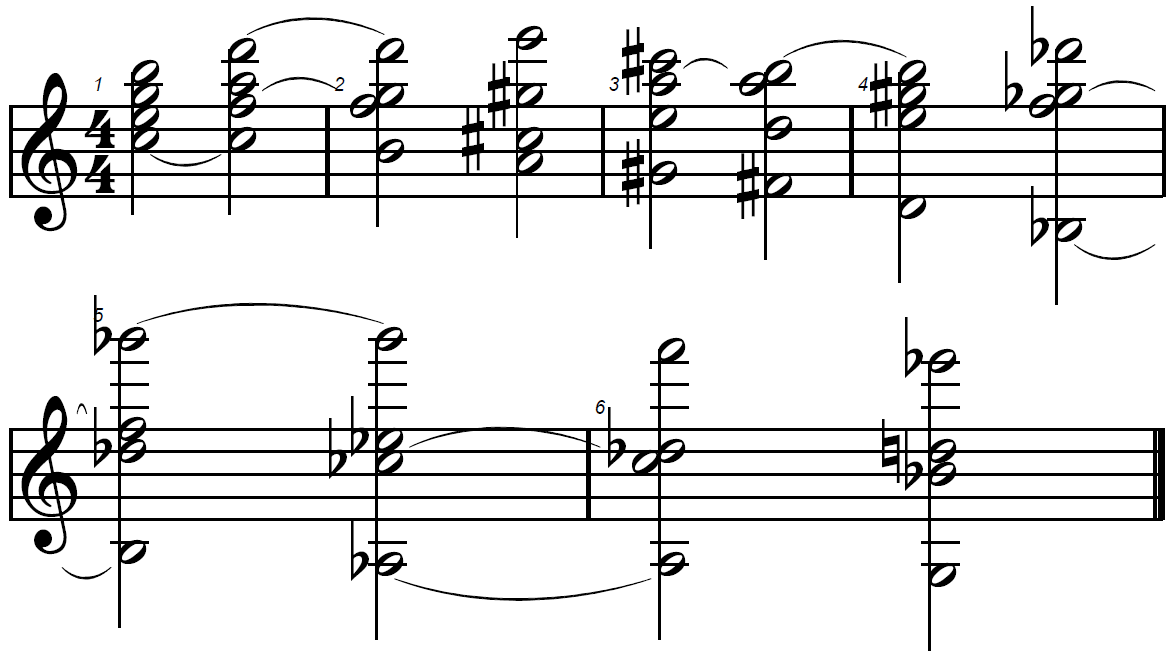
\includegraphics[width=8.5cm]{sequence}
	\caption{\textbf{Sequence}}
	\label{fig:sequence}
\end{figure}

\item Table \ref{tab:vcommands} and Figure \ref{fig:vcommands} show how the \texttt{V} commands can move voices one at a time to produce arbitrary counterpoint. In the Lindenmayer system's interpreter, voices with the same pitch in different chords are tied. In this system, the replacement rule for \texttt{B} itself includes references to \texttt{B}, so that 2 iterations cause a recursive expansion of the motive. The \texttt{T} commands also cause the 2nd replacement to move at a faster tempo.

\begin{table}[tbp]
\begin{tabular}{l|p{12cm}}
\hline
Iterations & 2\\
Axiom & \ttfamily C=CM7 B \\
Replace \ttfamily B & \ttfamily Td1.125 Cv Va0,2 Cv Va1,3 Va2,2 Cv B Vs3,4 Cv B Va0,2 Cv Va1,3 Va2,4 Cv Va3,3 Cv Cv Tm1.125\\
\hline
\end{tabular}
\caption{\textbf{Independent Voices}}
\label{tab:vcommands}
\end{table}

\begin{figure}[htbp]
	\centering
		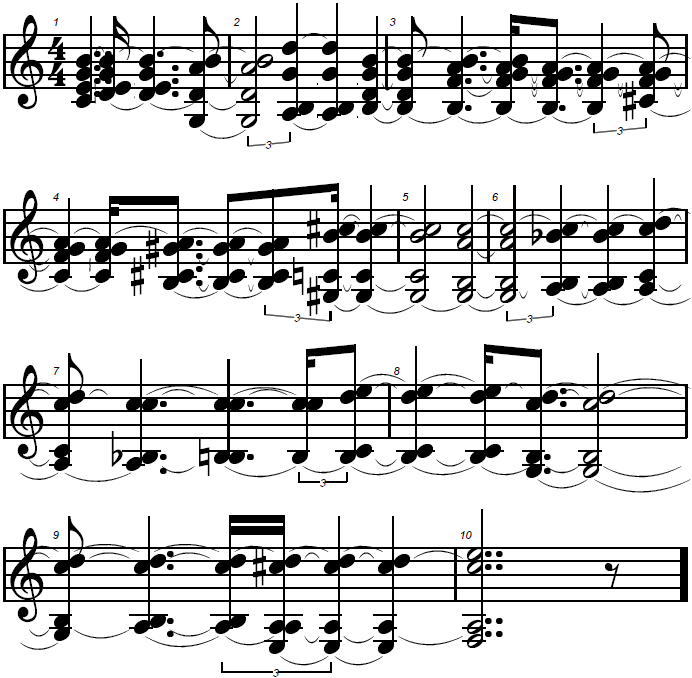
\includegraphics[width=8.5cm]{vcommands}
	\caption{\textbf{Independent Voices}}
	\label{fig:vcommands}
\end{figure}

\newpage

\item Finally, Table \ref{tab:samplepiece} represents the Lindenmayer system for a piece of 3 minutes 45 seconds. The axiom creates a major $7^{th}$ chord, then specifies an $A B B' A$ form. The $[$ and $]$ commands push and pop the turtle state from a stack, so that the chord appearing before $[$ re-appears after $]$. The $A$ section is constructed from the Table \ref{tab:sequence} sequence above, as well as another similar sequence. The $B$ section consists of the independent voices section described in Table \ref{tab:vcommands}, recursively constructed at faster and faster tempos. In the $B'$ section, one of the voices is moved before rule $B$ is applied, which affects all subsequent voice-leading. At the ends of the $A$, $D$, and $F$ sections, the $E$ section generates arpeggiations within some chords. 

\begin{table}[tbp]
\begin{tabular}{l|p{12cm}}
\hline
Iterations & 3\\
Axiom & \ttfamily C=CM7 V=4,0 V=5,1 V=6,2 V=7,3 A Cv Cv [ V=4,4 V=5,5 V=6,6 V=7,7 B Cv Cv B Cv Cv ] A Cv Cv\\
Replace \ttfamily A & \ttfamily F F E D D E F E Cv Cv\\
Replace \ttfamily B & \ttfamily Td1.125 Cv Va0,2 Cv Va1,3 Va2,2 Cv B Vs3,4 Cv B Va0,2 Cv Va1,3 Va2,4 Cv Va3,3 Cv Cv Tm1.125\\
Replace \ttfamily D & \ttfamily Cv Pv1,2,1,2 Cv Pv2,3,2,3 Cv D Cv\\
Replace \ttfamily E & \ttfamily Cv [ V=4,4 V=5,5 V=6,6 V=7,7 Td2. Vs3,12 Ca Vs2,12 Ca Vs1,12, Ca Vs0,12 Vs1,12 Vs2,12 Vs3,12 Ca E Tm2.0 ] Cv\\
Replace \ttfamily F & \ttfamily Cv Pv1,2,1,2 Cv Pv5,5,5,6 Cv Pv2,2,3,2 Cv F Cv\\
\hline
\end{tabular}
\caption{\textbf{Sample Piece}}
\label{tab:samplepiece}
\end{table}

\end{itemize}

\section{Discussion}

\subsection{Limitations}

\begin{itemize}

\item This approach knows something about voice-leading and chord progression.

\item This approach knows nothing about counterpoint proper, imitative procedures, tonal key, or serial procedures.

\item These spaces always represent a fixed number of voices, though dropping voices can be simulated by doubling or silencing some. 

\item The voice-leading algorithm is inflexible; the target chord stays close to the source chord in range, yet may wander up and down the score, or widen or narrow in range. 

\item In short, basic movements within musical spaces do not model the fine points of musical hearing or of any musical style.

\end{itemize}

\subsection{Strengths}

\begin{itemize}

\item One reader of an earlier version of this noted that the operations described here could have been implemented any number of ways --- why, therefore, do I feel that this geometric approach is better? 

\item I think it is better because representing chords as points makes it possible to represent all time and pitch information in any score as a function from time onto voice-leading space, or onto chord space. 

\item This in turn makes it easy to manipulate \emph{all} the time and pitch information in a score recursively (as with the Lindenmayer system), or even globally, using purely mathematical operations.

\item To me, the most interesting musical advantage of this system is how easily recursive patterns of movement in chord space can create top-down, hierarchical pitch structures of arbitrary depth.

\end{itemize}

\section{Future Directions}

\begin{itemize}

\item It should be easy to modify the voice-leading algorithm to control range and spacing.

\item It would be useful to have a concise way to represent changing numbers of voices.

\item These procedures are not complex, but in the context of algorithmic composition their very simplicity is a virtue, enabling the concepts to be adapted to a wide variety of compositional procedures. These could include:

\begin{itemize}

\item Chaotic dynamical systems

\item Applying musical filters to images or scientific data

\item Xenakis sieves or other stochastic generators

\item \emph{et cetera}

\end{itemize}

\item The use of geometry to model voice-leading and chords opens the composition of pitch structures up to all the resources of geometric algebra, and perhaps even topology and algebraic geometry. My impression is that these branches of mathematics have not seen as much musical application as, say, group theory.

\item There are a number of ways that chord space can be factored into subspaces. I am evaluating several different sets of subspaces regarding their suitability as geometric bases for atomic operations in algorithmic composition.

\end{itemize}

\section {Acknowledgments}

\begin{itemize}

\item I thank Dmitri Tymoczko for his generous patience in discussion and for helping me with the mathematics. 

\item I also benefitted from discussing earlier stages of these ideas with Drew Krause and the members of the New York Csound Users Group.

\item Any errors that remain here are of course my own. 

\end{itemize}


\bibliographystyle{chicago}
\small{
\bibliography{gogins}
}

\end{document}
